\documentclass[a4paper,10pt]{article}
% compile with pdflatex




% Package =====================================================================
\usepackage{graphicx} % used to insert the figure
\usepackage{multirow} % used for the table
\usepackage{geometry}
\usepackage[francais]{babel} % the language of the conference francais
\usepackage[utf8]{inputenc}
\usepackage[T1]{fontenc}
\usepackage{hyperref}
\hypersetup{pdfborder = 0 0 0} % pas de bordure autour des liens
\usepackage{subfigure}
\usepackage{sistyle}% for better and easy units (e.g. "\SI{25}{m.s^{-2}}")	
\usepackage{amsmath}


% New Command ===============================================================
\newcommand{\ud}{\mathrm{d}}
\renewcommand{\i}{\mathrm{i}}


% Style =====================================================================
% modification des marges
%\addtolength{\textwidth}{4cm}	% augmenation de la largeur du texte vers la droite
%\addtolength{\hoffset}{-2cm}	% marge associe gauche (=-0.5*textwidth) 		
\addtolength{\textheight}{2cm}% augmenation de la hauteur du texte vers le bas
%\addtolength{\voffset}{-1cm}  % marge associe haut (=-0.5*textheight)
\pagestyle{headings}

\title{\texttt{FindZerom} : A \textsc{Matlab} package for computing the roots of analytic functions}
\author{Benoit Nennig}
\date{Institut sup\'erieur de m\'ecanique de Paris (SUPMECA),\\ Laboratoire Quartz EA 7393,\\
3 rue Fernand Hainaut, 93407 Saint-Ouen, France.\\[0.5cm]
\url{benoit.nennig@supmeca.fr}\\[0.5cm]
\today}






% ==============================================================================
% ==============================================================================
\begin{document}



\maketitle
\begin{abstract}
This package is suitable to compute the roots of an analytic function present inside a closed contour. There are numerous available numerical techniques for this purpose like Newton-Raphson method, Muller's method, the Secant method or the Nelder-Mead simplex method. All these techniques have in common that they all require initial approximations for the zeros to start the algorithm. The proposed implementation is based on the method called the Cauchy Integration Method  or the Argument Principle Method and allows to compute the number of zeros (including its multiplicity) of $f$ from contour integral.

This program was initially developed for poroelastic silencer applications\cite{Nennig:2010} in order to solved dispersion equation. The algorithm has been already used in other application fields (see \cite{Delves:1967,Chen:2000,Kravanja:2000} and the references therein) and we proposed here a basic numerical implementation in matlab language.

This \emph{short} documentation explains quickly the theoretical background, shows the calling sequence and presents some examples of applications and validations.

This program is distributed in the hope that it will be useful, but WITHOUT ANY WARRANTY; without even the implied warranty of    MERCHANTABILITY or FITNESS FOR A PARTICULAR PURPOSE.  See the GNU General Public License for more details.

\end{abstract}


% ==============================================================================
\section{The winding number}
% ==============================================================================
% This technique is based on integration in the complex plane and can be used to solve the dispersion equation of a multilayer planar optical waveguide
% The method is often called the Cauchy Integration Method (CIM) or the Argument Principle Method (APM).
% pole 
The root-finding technique presented here is based on integration in the complex plan that does not require knowledge of initial guesses. 
The other advantages of the method is to avoid to evaluate at the function close to its root where round-off error may be important because of large dynamic of function obtained from matrix determinant. The roots are deduced from the regularity of the function away from the roots.

This is possible because of the Cauchy's Theorem, that allows to compute the number of zeros (including its multiplicity) of $f$  from the following
integral relation
\begin{equation}
    \label{eq:Arg_principle}
 S_0 = \frac{1}{2\pi \i} \oint_C \frac{f'(\beta)}{f(\beta)}  \ud \beta =
 \sum_{k=1}^{N_\beta} n_{k},
\end{equation}
where $N_\beta$ is the number of zeros and $n_{k}$ the corresponding multiplicity of the $k$-th
zero lying in the interior of the closed curve $C$. Note $f$ is chosen to be analytic
for the result to hold but the presence of poles may be included
by modifying the formula accordingly.
This is a classical procedure based
on the generalization on the previous relation to any monomial $\beta^n$, that is
~\cite{Kravanja:2000}
\begin{equation}
    \label{eq:windingNumber}
S_n = \frac{1}{2\pi \i} \oint_C \frac{f'(\beta)}{f(\beta)} \beta^n \ud \beta =
 \sum_{k=1}^{N_\beta} n_{k} \beta_{k}^n,
\end{equation}
where $\beta_{k}$ denote the position of the $k$-th zero.
To simplify further the analysis, function $f$ is assumed to
have only simple zeros so the integral \eqref{eq:Arg_principle} is exactly the number of zeros contained in the interior of $C$. Note this is not a stringent assumption as the occurrence of multiple zeros is highly improbable
(in a somewhat different context, it is known that multiplicity may exist
for specific material properties set for which simple zeros are merging \cite{Nilsson:1980,Bloch3D:20107}).
We now introduce the associated polynomial $\Pi$ for the interior of $C$, that is
a polynomial having the same zeros as $f$, i.e.
\begin{equation}
\label{eq:Pi}
    \Pi(\beta) = \prod_{k=1}^{N_\beta} ( \beta - \beta_{k}) = \sum_{n=0}^{N_\beta} C_n \beta^n.
\end{equation}
Of course the zeros are not known yet, but the polynomial coefficients $C_n$
can be efficiently computed from the following recursive algorithm~\cite{Cristini:1994,Chen:2000}
\begin{equation}
    \label{eq:Cn}
    C_n = \left\{ \begin{aligned}
    &1, &        & \text{if } n=S_0\\
  &\frac{1}{n-S_0}\sum_{j=1}^{S_0-n} S_j \,  C_{n+j},     &   & \text{if } n = S_0-1, \ldots, 0.
    \end{aligned} \right.
\end{equation}
Here $S_n$ ($n=0,1,2,\ldots,N_\beta$), denote the values of the integral \eqref{eq:windingNumber}.
Once $\Pi$ is known, finding its zeros simply requires computing  the eigenvalues of the companion matrix which is a very fast procedure for moderate size matrices.



%%%%%%%%%%%%%
%Let $f(z)$ be a meromorphic function defined inside and on a simple closed contour $C$, with no zeros or poles on $C$. Applying the Cauchy Residue Theorem yields
%\begin{equation}
%	\label{eq:windingNumber}
%S_n = 	\frac{1}{2\pi \i} \oint_C \frac{f'(z)}{f(z)} z^n \ud z = \sum_{k=1}^{N_z} n_{z_k} z_{z_k}^n - \sum_{j=1}^{N_p} n_{p_j} z_{p_j}^n.
%\end{equation}
%Where, $n_{z_k}$ and $n_{p_j}$ are $k^{\mathrm{th}}$ zeros and $j^{\mathrm{th}}$ pole multiplicity and $z_{p_k}$ and $z_{z_j}$ their position. Finally, the integer $N_z$ and $N_p$ denote the number of zeros and poles. 
%If, $D(\beta)$ has no pole and $N_z=0$, the zeros multiplicity is always one excepted for certain properties set were zeros may collapse~\cite{Nilsson:1980,Bloch3D:2017}. If $n$ is fixed to 0 and if the poles are out of the integration contour $C$, Eq.~(\ref{eq:windingNumber}) gives the number of zeros include in $C$. This quantity is know as the winding number or argument principle. Most authors used this expression to ensure they do not miss any roots. 
%Using Eq.~(\ref{eq:windingNumber}) and various value of $n$ the equivalent polymon $q(z)$ which has the same root as $f$ can be built~\cite{Cristini:1994,Chen:2000,Kravanja:2000}
%\begin{equation}
%\label{eq:q(z)}
%	q(z) = \prod_{i=1}^{S_0} \left( z - z_{z_i} \right) = \sum_{k=0}^{S_0} C_k z^k,
%\end{equation}
%where 
%\begin{equation}
%	\label{eq:Ck}
%	C_k = \left\{ \begin{aligned}
%	&1, &        & \text{if } k=S_0\\
%  &\frac{1}{k-S_0}\sum_{j=1}^{S_0-k}S_j C_{k+j},     &   & \text{if } k = S_0-1, \ldots, 0.
%	\end{aligned} \right.
%\end{equation}
%To increase speed in Matlab environment an non-recursive implementation of Eq.~(\ref{eq:Ck}) is preferable. Then $q(z)=0$ is solved by computing the eigenvalues of the companion
%matrix~\cite{Edelman:1995}.
%In the following of this paper, we shall assume that $D(\beta)$ is a meromorphic function.  Even if this is generally the case for a wide panel of wave guides with finite cross section, the proof is tedious considering the complexity of analytical expression of $D(\beta)$. In addition, as the winding number gives rise to accurate results, presented in section~\ref{sec:Conv}, this assumption seen to be valid.


More details can be found in \cite{Kravanja:2000} and many other applications can be found in the reference listed therein of in Refs.~\cite{Chen:2000,Nennig:2010}. Note that extension are possible to matrix functions\cite{Guttel:2017,SLEPc}.


\subsection{Numerical Implementation}
% ==============================================================================

% différence finis, ordre
% factorisation de R^n
% couronne
% cercle élippse

The most time consuming operation is the numerical evaluation of the functions with complex arguments at some quadrature
points when  computing integrals \eqref{eq:windingNumber}.
Since these are integrals of an analytic periodic function over a complete period, the trapezoidal rule is the optimal quadrature rule\cite[25.4.3]{Abramowitz:1965}. Let $C$ be defined from a regular function $\gamma(s)$ over the interval $s \in [0,2\pi]$, then the $q$-point trapezoidal rule approximation to $S_n$ is given by
\begin{equation}
S_n \approx \frac{1}{\i q} \sum_{i=0}^{q-1} \left ( \frac{\gamma^n}{\hat{f}}
\frac{\ud \hat{f}}{\ud s} \right ) (i/q),
\end{equation}
where we put $\hat{f}(s)=f(\gamma(s))$. Though the $s$-derivative of $\hat{f}$ may
be obtained formally via symbolic software, it is far more efficient to evaluate
the derivative using high order central finite difference scheme, that is
\begin{equation}
\frac{\ud \hat{f}}{\ud s} (i/q) \approx \frac{1}{i/q} \sum_{j=-J}^{J} a_{|j|} \hat{f} \left(\frac{i+j}{q}\right).
\end{equation}
The procedure is extremely fast since the discrete values  of $\hat{f}$ on the regular grid
are already calculated.
 Here we used either the $5^{\mathrm{th}}$ or $9^{\mathrm{th}}$-order scheme.
 The corresponding coefficients are displayed  in Table~\ref{tab:FiniteDifferenceSchemeCoefficients}.
 \begin{table}[htbp]
    \centering
    \caption{Finite difference scheme coefficients.}
        \begin{tabular}{lccccc}
        \hline
\hline
                              & $a_0$  &    $a_1$    &    $a_2$    & $a_3$    & $a_4$   \\
        \hline
\rule{0pt}{3ex}$5^\mathrm{th}$ order &   0    &     2/3     &     -1/12   &    -     &   -      \\
        $9^\mathrm{th}$ order &   0    &     4/5     &    -1/5     &  4/105   &  -1/280 \\
\hline
\hline        
        \end{tabular}      
    \label{tab:FiniteDifferenceSchemeCoefficients}
\end{table}
The choice of the curve $C$ must depend upon the region of the complex plane where
eigenvalues are searched. When roots are expected to be symmetric
with respect to the origin, choosing the circular path $\gamma=a \mathrm{e}^{\i s}$
appears to be a good compromise.
To avoid possible round-off errors, it is then preferable to factorize the
term $a^n$ and exclude it for the trapezoidal summation of Eq.~(\ref{eq:windingNumber}).
Now, if the roots are concentrated along the real or the imaginary axis, elliptical contour integration may also be used. In this case we take $\gamma= a \cos s + \i b \sin s$. To conserve good convergence properties in the trapezoidal rule, smooth contour are highly recommended (use reasonable aspect ratio in the ellipse).



%
%The most time consuming operation is the evaluation of  $D(\beta)$ for each $\beta$ of $C$, so everything must be done to limit the evaluation number $N_C$. For this reason high order central finite  difference scheme are used to evaluate the $z$-derivative of $D(\beta)$ because the evaluation points of $D(\beta)$ can be reused. As the integration contour is periodic their is no hindrance to used this kind of scheme, sometime handicapped by domain ends. Here we used the 9$^{\mathrm{th}}$-order scheme presented in Eq.~(\ref{eq:FD}) and in table~\ref{tab:FiniteDifferenceSchemeCoefficients}, which provides some enhancement if $N_C$ is very low. Before applying this scheme, we need to replace the $z$-derivative by $\theta$-derivative. The chain rule leads to
%\begin{equation}
%\frac{\partial D}{\partial z} = \frac{1}{z\i} \frac{\partial D}{\partial \theta}, \quad \text{with }z=R \mathrm{e}^{\i \theta},
%\end{equation}
%and
%\begin{equation}
%	\label{eq:FD}
%	\frac{\partial D}{\partial \theta} \approx \frac{1}{\Delta \theta} \sum_{i=-N}^N a_i \, D_{i}, \quad \text{with } \quad a_i = a_{-i}.
%\end{equation}
%Here, $D_i$ denotes the dispersion equation evaluated at the $i^\mathrm{th}$ node of the stencil and $\Delta \theta$ is the angular-grid spacing. 
%Then, trapezoidal integration rule is applied to Eq.~(\ref{eq:windingNumber}) because of is exponential convergence on periodic function\cite[25.4.3]{Abramowitz:1965}. To avoid round off error, it is preferable to factorize $R^n$ and exclude it for the trapezoidal summation of Eq.~(\ref{eq:windingNumber}).
%As zeros are located near the imaginary axis, elliptical contour integration can also be used. In this case, $z= R_1 \cos {\theta} + \i R_2 \sin{\theta}$. If the ellipse is not to flat, the same convergence properties may be hope.

%because the shape of integration contour should remain very smooth to keep the good convergence of the trapezoidal integration rule of Eq.~(\ref{eq:windingNumber}).

%\begin{table}[htbp]
%	\centering
%	\caption{Finite difference scheme coefficients}
%		\begin{tabular}{lccccc}
%		\hline
%		                      & $a_0$  &    $a_1$    &    $a_2$    & $a_3$    & $a_4$   \\
%		\hline
%\rule{0pt}{3ex}$5^\mathrm{th}$ order &   0    &     2/3     &     -1/12   &    -     &   -      \\
%		$9^\mathrm{th}$ order &   0    &     4/5     &    -1/5     &  4/105   &  -1/280 \\			
%\hline
%		\end{tabular}
%
%	\label{tab:FiniteDifferenceSchemeCoefficients}
%\end{table}





The numerical results accuracy can be check because \eqref{eq:Arg_principle} provides the number of zeros. If the number is not closed to an integer, the algorithm has encountered some trouble e. g. 
\begin{itemize}
\item Presence of non analytic functions (tangent, some bessel function ratio, square root\dots)
\item Too few points
\item A zeros is located on the contour
\end{itemize}
The algorithm change slightly the radius (see variable \texttt{RShift}) of the integration path and start again.

%Important to use integer number of sample on the integration path
The proposed implementation was relevant for our application. Other approaches can also be used for instance use logarithm instead of the ratio $f'/f$, use orthogonal polynom basis\dots


\paragraph{remarks}
If needed, pole can be easily remove by creating a hole in the integration contour. The multiplicity can be obtained but it is not implemented for now. When exponential growth becomes a problem, it is sometime possible to provide directly the ratio $f'/f$ instead of computing $f$ and $f'$ separately.




\subsection{Convergence} \label{sec:Conv}
% ==============================================================================
% verif si entier pour éviter que le zeros ne soit trop près du contour.

Here are exposed some practical tips to set up the root-finding parameters to get cheaply the required accuracy on $\beta$'s.
It's worth noting that the more zeros are present in the integration path, the more the dynamic of polynom coefficients $C_k$ is large and subject to round-off error. The repercussion on the roots location may be significant. 
The solution used here is to split the integration path into concentric ring ; data coming from the previous path can be obviously store. 
This remarks are illustrated in Table~\ref{tab:ConvergeWaveNumber}. A single circular/elliptical integration contour leads to poor results if more than 15 zeros are present because the round-off stop the convergence. In return, with the same number of $D(\beta)$ evaluation ($N_C/2$ for each circle), the two step approach is by far better. In our application $N_C \in [ 500,1000]$ is a good compromise between time and accuracy.
This method is sometime faster than doing a refinement, with a small circle or using an other algorithm, for each zeros
given by a first rough calculation. Nonetheless, the local refinement is present in the package.
%


\begin{table*}[htbp]
	\centering
	%\begin{scriptsize}
		\caption{Converge of one wave number at fixed integration radius $R=180$ at 1730 Hz for XFM foam. With one circular integration path (left) and with one circular and annular path (right). Bold character denotes the good digit (extract from Ref~\cite{Nennig:2010}).}
		\begin{tabular}{rrrr}
		\hline
\multicolumn{2}{c}{$N_{z} = 20$} & \multicolumn{2}{c}{$N_{z} = 10 + 10$}\\
		\cline{1-2} \cline{3-4}
		\multicolumn{1}{c}{$N_C$\rule{0pt}{3.5ex}}     &    \multicolumn{1}{c}{$\beta$}     & \multicolumn{1}{c}{$N_C$}  &       \multicolumn{1}{c}{$\beta$}\\
\rule{0pt}{4ex} 500      & \textbf{1}8.1310333520   + \textbf{1}7.2414041458 $\i$     & 500&    \textbf{17}.1619265538  +  \textbf{15}.2060360731 $\i$\\
		            1000     & \textbf{17.6}094544451   + \textbf{1}4.9503659291 $\i$     & 1000&    \textbf{17.62934}56921   + \textbf{15.065}0726700 $\i$\\
		            5000     & \textbf{17.6}308169754   + \textbf{15.0}352734983 $\i$     & 5000&    \textbf{17.6294474640}   + \textbf{15.065151316}3 $\i$\\
		            20000    & \textbf{17.6}362164376   + \textbf{15.0}289704442 $\i$     & 20000&   \textbf{17.6294474640}   + \textbf{15.0651513164} $\i$ 		\\
		            \hline
		            \end{tabular}
		
%		\end{scriptsize}
	\label{tab:ConvergeWaveNumber}
\end{table*}

To get 6 figures on 20 roots, around 1000 function was required. This leads to around 50 function evaluations per roots. This is a good results when compare to the complexity of the problem from Ref~\cite{Nennig:2010}.



% ==============================================================================
\section{Package matlab}
% ==============================================================================
The package is built on three main file
\begin{itemize}
\item \texttt{FindZerosm.m}, the main routine
\item \texttt{diffZcircleTheta.m}, use compute high order finite differences
\item \texttt{CoefC}, to recast the coeficients $S_n$ into the suitable polynomial form.
\end{itemize}
this files are adapted to handle elliptic integral path :\texttt{diffZcircleEllipse.m}. The calling syntax is recalled here
\begin{verbatim}
[K, *Ci] = FindZerosm(R,N,fhandle, *Refine, *R0)
% Mandatory input args :
%  R : integration radius
%  N : number of integration points
%  fhandle : finds the zero of the anonymous function fhandle
% Optionnal input args (indicated by *) :
%  Refine = 1 ou 0 (local refinement with small circle around each root)
%  R0 = 0 si l'origine est en O, coordonée de l'origine sinon
% Mandatory output args :
%  K : roots
% Optionnal output args (indicated by *):
%  Ci : save of contour usefull value for annular computation
\end{verbatim}
If more than 15-20 zeros are present in $C$, it is often better to use annular contour to get the 15-20 roots in each closed contour.
\begin{verbatim}
[K1,Ci] = FindZerosm(R1,N,@nom, *Refine, *R0);                       % disk between 0 and R1
[K2,Ci] = FindZerosmAnnular(R2,N,@nom,Ci, *Refine, *R0);             % Annular region between R1 and R2
[K3,Ci] = FindZerosmAnnularEllipse([R3 R4],N,@nom,Ci, *Refine, *R0); % "Annular" elliptic R2 and [R3 R4]
K = [K1 ; K2 ; K3];
\end{verbatim}
Circular contour and elliptic contour are provided. %Ellipic contour are suitable if the roots are clustered to one axes.
%Enfin au lieu des couronnes il est aussi possible d'utiliser une version généralisée qui intrègre sur un contour élliptique. Elle est particulièrement utile si les zeros sont proche des axes. Attention toutefois à ne pas trop écraser l'ellipse, car l'intégration convergera moins vite (ou augmenter \texttt{N}).


% ==============================================================================
\section{Validation and examples}
% ==============================================================================


\subsection{Cantilever beam}
% ------------------------------------------------------------------------------
The first example concern a cantilever beam of length $L$. We are looking for the first discrete values of the wavenumber $\alpha_n$ roots of 
\begin{equation}
f(\alpha L) = \cos \alpha L \cosh \alpha L -1.
\end{equation}
The roots can be used for instance to compute the eigenfrequency of the beam. The usefull root are real and positive value of $\alpha_n L$.

For a complete problem description, see \url{https://en.wikipedia.org/wiki/Euler-Bernoulli_beam_theory}. For an illustration of the package see \texttt{example/Cantilver.m}.

\subsection{2D acoustic liner dispersion equation}
% ------------------------------------------------------------------------------
The second proposed example (time convention $\mathrm{e}^{-\omega t}$) is based on acoustic propagation in a duct of height $h$ lined with an impedance. The dispersion equation reads
\begin{equation}
	g(\alpha) = \alpha \tan \alpha h + \frac{\i k}{Z}.
\end{equation}
The roots are the transverse wavenumbers $\alpha_n$ and are related to the axial wavenumber with the relation $k^2 = \beta_n^2 + \alpha_n^2$, where $k$ is the free field wavenumber.

To use the proposed method, the previous equation must be modified to keep analytic function 
\begin{equation}
	f(\alpha) = \alpha \sin \alpha h + \frac{\i k}{Z} \cos \alpha h.
\end{equation}
To the authors best knowledge, this always possible for closed waveguides.



The proposed approach is validated with the results from Fig.~\ref{fig:sri} extracted from \cite{ when $h=1$, $k=1$, $c_0=1$ and $Z=3.5(1+\i)$ in \texttt{example/Liner2D.m} obtained with Newton-Raphson method.


%
%\begin{equation}
%\cos{\alpha h}+ \frac{Z\i \alpha }{\omega \rho_0} \sin{\alpha h} =0.
%\end{equation}
%Cette expression est obtenue directement en calculant le déterminant de la matrice si les conditions sont écrites avec les exponentielles.

%Pour que la méthode marche la fonction $f$ doit être méromorphe. Passer par la fonction tangente ne le permet pas.

\begin{figure}\label{fig:sri}
	\centering
		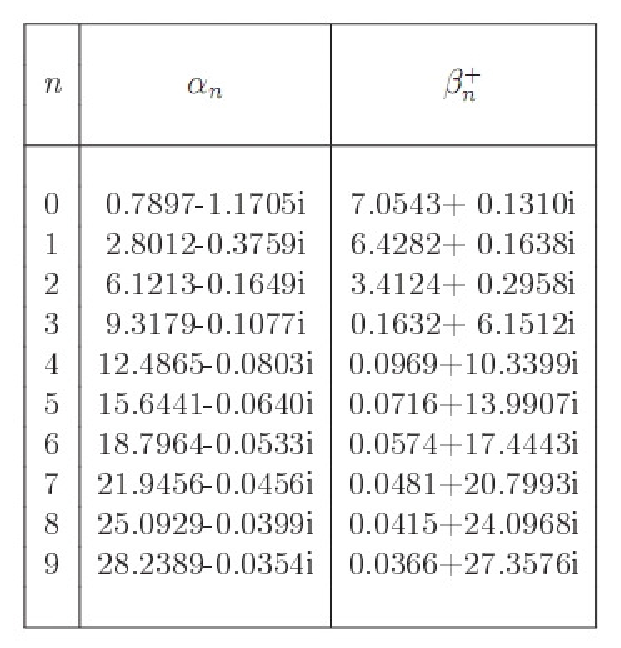
\includegraphics[width=0.50\textwidth]{sri.pdf}
	\caption{Example of numerical values\cite{Poernomo:2008} for transversal and axial wavenumber obtained for a lined 2D acoustic duct, $k=7$, $h=1$, and $Z=\pm 3.5(1+1i)$ obtained with Newton-Raphson method.}
	\label{fig:sri}
\end{figure}

For this particular example,  $R=10$ and 500 points are put along the contour $C$ . All figures are the same and the computation time is around 0.02 seconds.



% BIBLIO ===============================================================================
\bibliographystyle{plain}
\bibliography{biblio}
% http://www.chebfun.org/examples/roots/ComplexRoots.html see also
\end{document}
